Here we will explain how we developed our AXI interconnect, first explaining how it works as a stand-alone component, and then how we inserted it into the Processor.
\newline

{\color{Blue}{\subsection{Block Design}}}
In the figure \ref{HLBD} is reported the Block Diagram of the AXI interconnect we developed.
\newline
What we have implemented is essentially the {\bf crossbar}-related part inside the {\bf original AXI interconnection}: we specifically tailored our component to fit in the ARM Design Start, so {\bf single-master multiple-slaves architecture}, but with few changes the number of slaves can be increased/decreased.
\newline
The architecture is divided into {\bf two independent} mirrored {\bf parts}, one for the {\bf write} operation and one for the {\bf read} operation, that are differentiated only by the inner logic of the two FSMs and by the number of wires that they manage. Their core is the {\bf MUX-DEMUX-DECODER} sub-units for the {\bf routing} of the signals and a supporting {\bf FSM for} the handling of {\bf handshakes}.
\newline
The \underline{MUX} / {\it DEMUX} simply gathers the messages \underline{from slaves to master} / {\it from the master to the slaves} and \underline{rally them for the master} / {\it redirect them to the correct slave} under the explicit command of the {\bf DECODER} that {\bf maps the components} upon their {\bf addresses}.
\newline
The FSM is in charge to follow the master in the write/read operations: it tracks the sequence of handshake (address -> data for read and address -> data -> response for write) keeping frozen the MUX / DEMUX states to preserve the connection of the interested parts of the system.
\newline
There are 2 types of error that we had considered: the ones raised by the slaves, which merely pass through the inteconnection and the ones raised if the address of the required slave is not mapped. The {\bf FSM} is also a {\bf supervisor} in case of the {\bf errors} in the {\bf addressing}: if the DECODER detects that the address provided by the master is not valid, the FSM will commute to an {\bf error-handling state} and allow the AXI to show an appropriate behaviour.
\newline

\begin{figure}[h]
  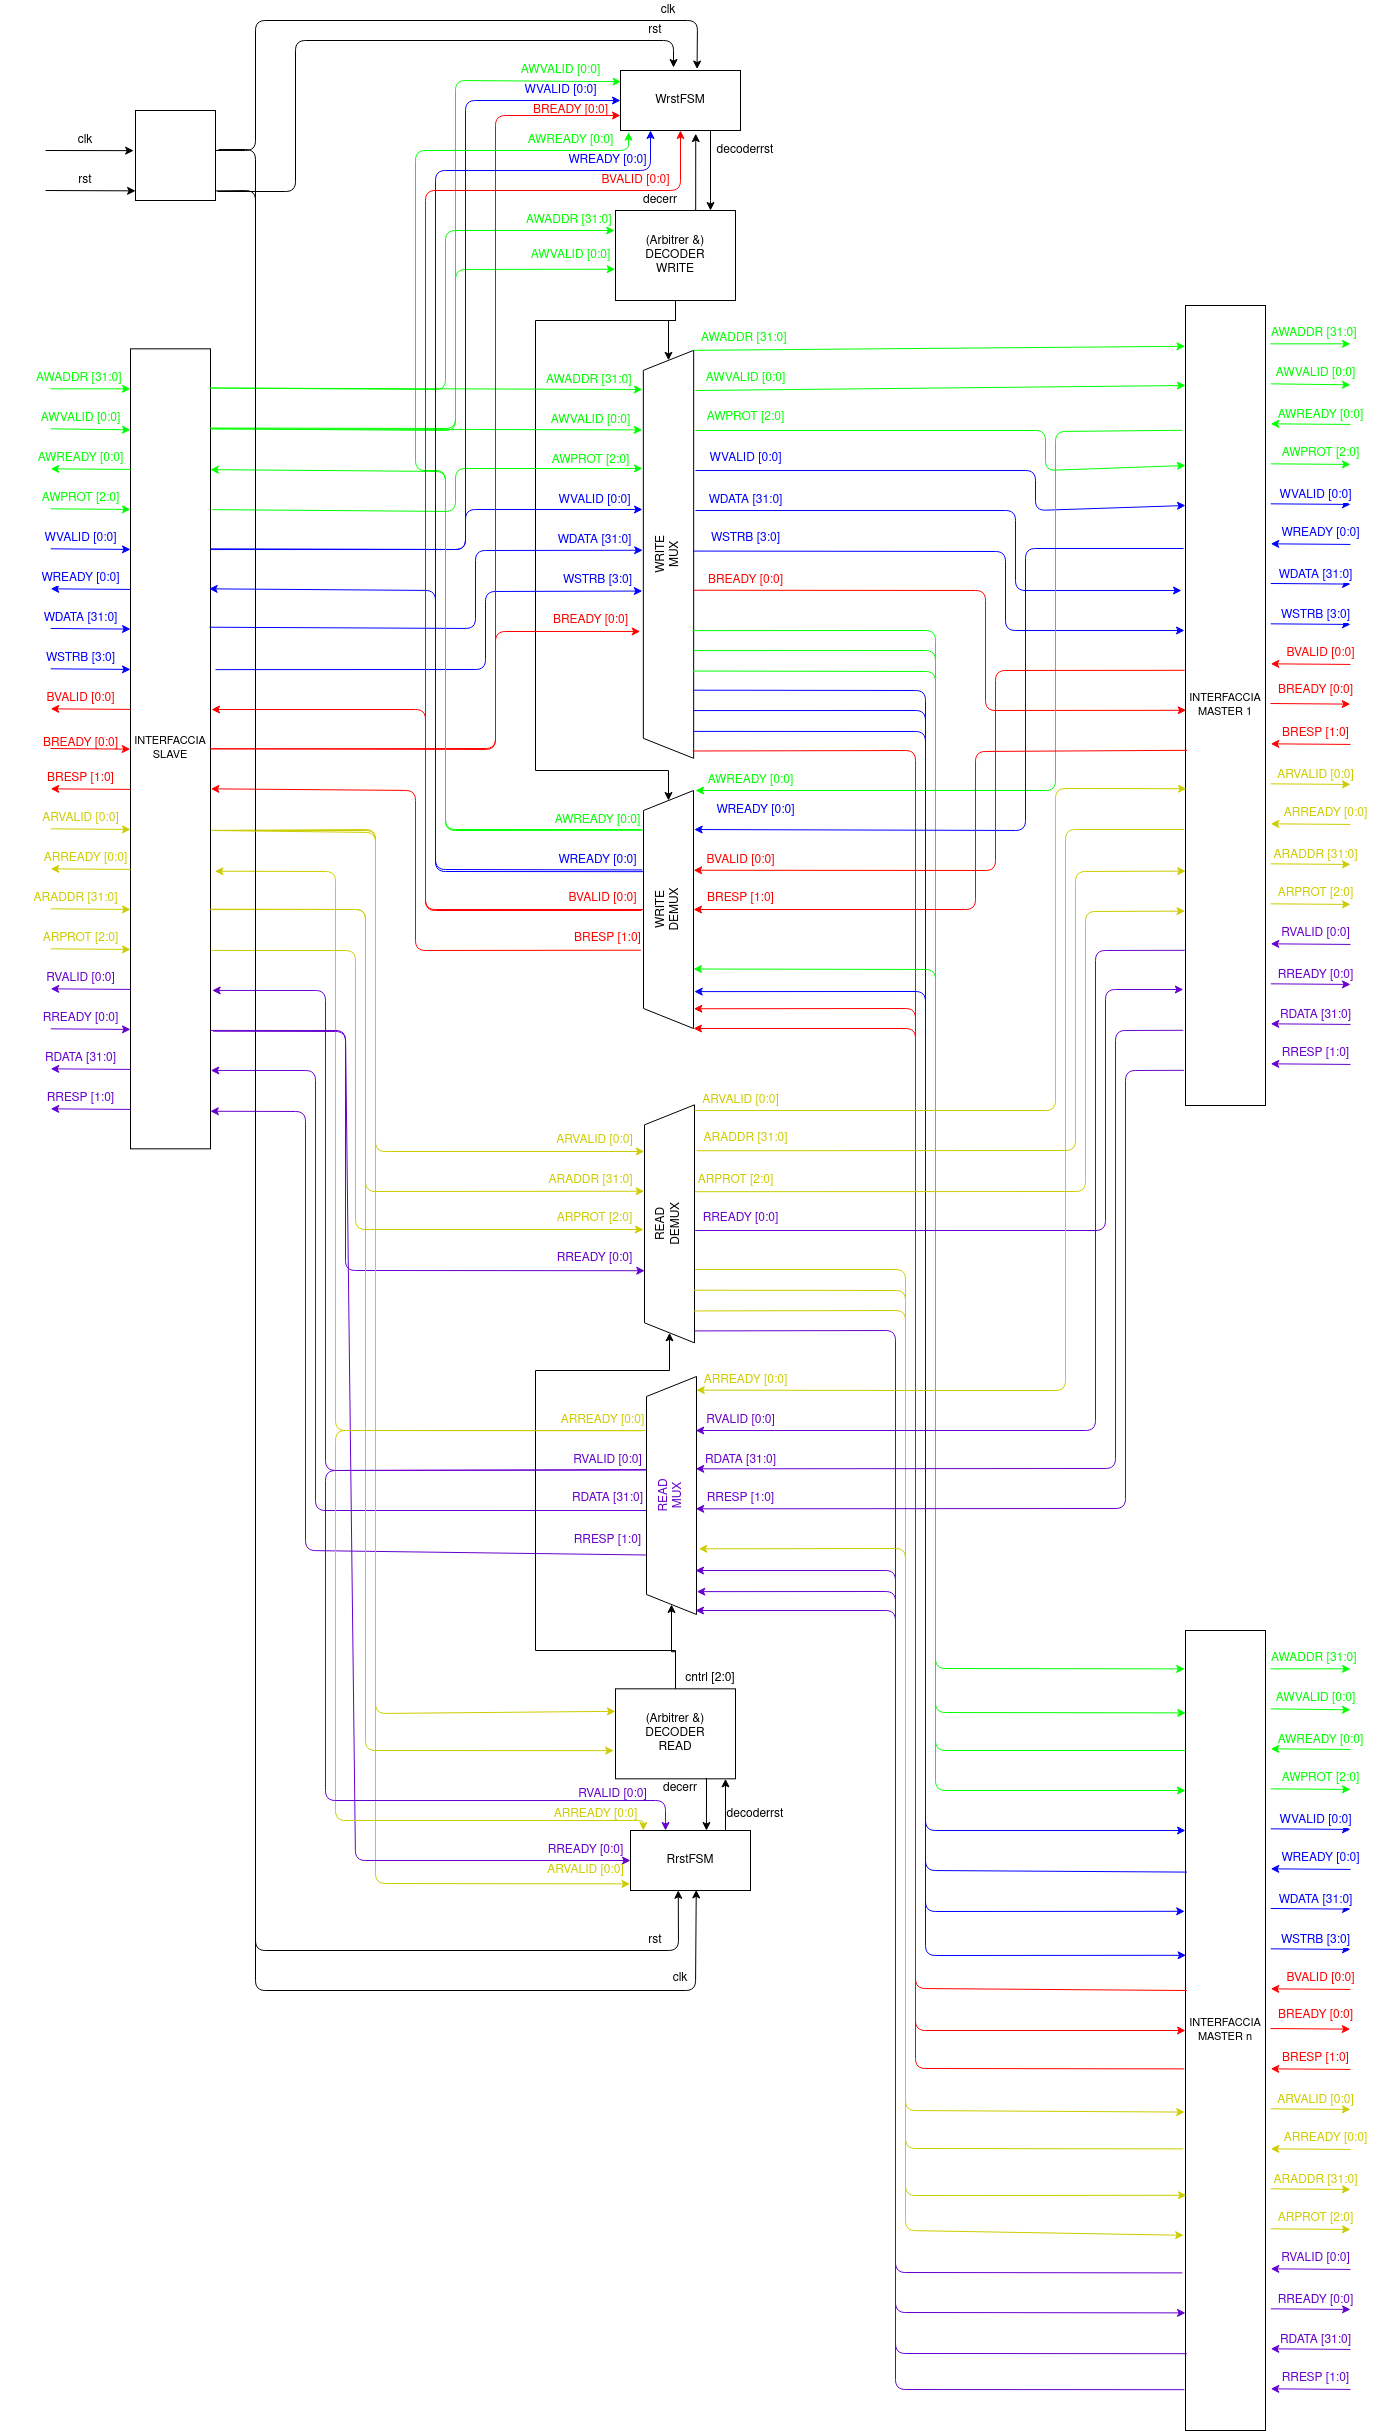
\includegraphics[width=0.9\textwidth, angle=0]{"./../../img/Images/highLevel.png"}
  \caption{highLevel block diagram}
  \label{HLBD}
\end{figure}

{\color{Blue}{\subsection{Integration and Testing}}}
 We preferred to use the same enviroment of {\bf ARM Design Start} respect to the implementation of a fake memory to {\bf test the correctness} of our design: we make this choiche to make a {\bf comparison between the original wave diagram} and the {\bf one produced} with {\bf our AXI} in. Aside from our component, we have had to insert an {\bf ad hoc adapter} to match the {\bf full AXI3} interface exposed by the processor to the {\bf AXI4-Lite} implemented by us.
\newline
